\documentclass[compress,mathserif,table,xcolor=dvipsnames,10pt]{beamer}
%%%%%%%%%%%%%%%%%%%%%%%%%%%%%%%%%%%%
% %Para imprimir: grande y sin pause
%\documentclass[compress,mathserif,table, hyperref={citecolor=olive}, handout]{beamer} 
% \usepackage{pgfpages}
% % \pgfpagesuselayout{2 on 1}[a4paper,border shrink=5mm] % dos pags vertical
% \pgfpagesuselayout{4 on 1}[a4paper,border shrink=4mm, landscape] % 4 pags horizontal
% \mode<handout>{\setbeamercolor{background canvas}{bg=black!5}}
%%%%%%%%%%%%%%%%%%%%%%%%%%%%%
% \usepackage[spanish,activeacute]{babel}
% \deactivatetilden
% \usepackage[latin9]{inputenc}
% \usepackage[spanish,activeacute]{babel}
\usepackage{latexsym}
\usepackage{setspace}
\usepackage{amssymb}
\usepackage{amsfonts}
\usepackage{mdwlist}
%\usepackage{proof} 
\usepackage{graphicx}
\usepackage{ulem} % para tachar
\usepackage{colortbl} % colores para las tablas

\usepackage{proof}
\usepackage{pifont}

\usepackage{tikz}
\usepackage{fancybox} %Ovalbox
\usepackage{stmaryrd}

% Comandos paco
\newcommand{\nc}{\newcommand}
\nc{\bframe}{\begin{frame}}
%\nc{\eframe}{\end{frame}}
\nc{\frt}{\frametitle}
\nc{\os}{\onlyslide} % esto es prosper
\nc{\uc}{\uncover}
\nc{\bcol}{\begin{columns}}
\nc{\ecol}{\end{columns}}
%
\nc{\muestra}[2]{\alert<#1>{#2}}
\nc{\bcboxby}[1]{\begin{beamercolorbox}[rounded=true]{fg=black,bg=yellow}{#1}\end{beamercolorbox}}
\nc{\bcboxbw}[1]{\begin{beamercolorbox}[rounded=true]{fg=black,bg=white}{#1}\end{beamercolorbox}}
\nc{\bcboxblw}[1]{\begin{beamercolorbox}[rounded=true]{fg=blue,bg=white}{#1}\end{beamercolorbox}}
\nc{\bcboxbbl}[1]{\begin{beamercolorbox}[rounded=true]{fg=black,bg=yellow}{#1}\end{beamercolorbox}}
% 
\nc{\coment}[1]{}
\nc{\primero}{$^{o}$}
\nc{\primera}{$^\mathrm{a}$}
\nc{\abreint}{?`}
% 
% abreviaturas
\nc{\bdoc}{\begin{document}}
\nc{\edoc}{\end{document}}
\nc{\bcen}{\begin{center}}
\nc{\ecen}{\end{center}}
\nc{\cen}[1]{\bcen #1 \ecen}
\nc{\bit}{\begin{itemize}}
\nc{\eit}{\end{itemize}}
\nc{\benum}{\begin{enumerate}}
\nc{\eenum}{\end{enumerate}}
\nc{\bdes}{\begin{description}}
\nc{\edes}{\end{description}}
\nc{\ba}{\begin{array}}
\nc{\ea}{\end{array}}
\nc{\btab}{\begin{tabular}}
\nc{\etab}{\end{tabular}}
\nc{\btabb}{\begin{tabbing}}
\nc{\etabb}{\end{tabbing}}
\nc{\bmp}{\begin{minipage}}
\nc{\emp}{\end{minipage}}
  
\nc{\tp}[1]{\overline{#1}}
\nc{\ul}{\underline}

\def\h#1{\hspace*{#1cm}}
\def\hh#1{\hspace*{0.#1cm}}
\def\v#1{\vspace*{#1cm}}
\def\vv#1{\vspace*{0.#1cm}}

\newcommand{\enfa}[1]{{\color{Red}#1}}

% Arrows
\newcommand{\lt}[2]{\leadsto^{#1}_{#2}}
\newcommand{\tn}{\to_{\mathit{norm}}}
\newcommand{\tred}{\to_{\mathit{red}}}
\newcommand{\st}{\Rightarrow^\mi{top}}
\newcommand{\q}[1]{\Rightarrow^{\texttt{#1}}}

% Hets
\nc{\Hets}{\textmd{\textsc{Hets}}\xspace}
\nc{\CASL}{\textmd{\textsc{Casl}}\xspace}
\nc{\CoFI}{\textmd{\textsc{CoFI}}\xspace}
\nc{\HetCASL}{Het\textmd{\textsc{Casl}}\xspace}
\nc{\rewrites}{\Rightarrow}
\nc{\SPASS}{\textmd{\textsc{Spass}}\xspace}
\nc{\rew}{\rewrites}

% Algunos marcadores
\nc{\mi}{$~\bullet~$}
\nc{\mii}{$~\star~$}
\nc{\miii}{$\rhd~$}
\nc{\miv}{\ -\ }

% Etiquetas Proof Trees
\newcommand{\lab}[1]{\mathsf{#1}}
\newcommand{\labapt}[1]{\!\scriptstyle\lab{#1}}

% Colors
\definecolor{emphcol}{rgb}{1,0,0} % red
\definecolor{green}{rgb}{0,1,0} % green
\definecolor{blue}{rgb}{0,0,1} % blue
\definecolor{white}{rgb}{1,1,1} % white

\nc{\col}[1]{{\color{structure}#1}}
\nc{\gr}[1]{{\color{green}#1}}
\nc{\wh}[1]{{\color{white}#1}}
\nc{\bl}[1]{{\color{blue}#1}}
\nc{\re}[1]{{\color{emphcol}#1}}

% K
\nc{\K}{$\mathbb{K}$\xspace}

% Flechas
\nc{\ra}{\rightarrow}
\nc{\Ra}{\Rightarrow}
\nc{\la}{\lefttarrow}
\nc{\La}{\Leftarrow}
\nc{\lra}{\leftrightarrow}
\nc{\Lra}{\Leftrightarrow}
\nc{\sii}{\Lra}
\nc{\vp}{\varphi}
\nc{\vacia}{\Box}
\nc{\landa}{$\backslash$}

\nc{\codtt}[1]{{\tt #1}}
\nc{\cod}{\codtt}

\nc{\codesize}{\small}

\graphicspath{{images/}}

%\nc{\den}[1]{[\![#1]\!]} % Corchetes semanticos

% Colores
\nc{\trgb}{\textcolor[rgb]}
\nc{\negro}[1]{\textcolor[rgb]{0.00,0.00,0.00}{#1}}
\xdefinecolor{olive}{cmyk}{0.64,0,0.95,0.4}
\xdefinecolor{morWai}{rgb}{0.50,0.00,0.50}
% \nc{\verdec}[1]{\textcolor[rgb]{0.00,1.00,0.00}{#1}}
\nc{\verdec}[1]{\textcolor{olive}{#1}}
\nc{\verdeco}[1]{\textcolor[rgb]{0.00,0.59,0.00}{#1}}
\nc{\verdeo}[1]{\textcolor[rgb]{0.00,0.25,0.00}{#1}}
\nc{\azulc}[1]{\textcolor[rgb]{0.00,0.00,1.00}{#1}}
\nc{\azulco}[1]{\textcolor[rgb]{0.00,0.53,0.68}{#1}}
\nc{\azulo}[1]{\textcolor[rgb]{0.00,0.00,0.50}{#1}}
\nc{\grisc}[1]{\textcolor[rgb]{0.50,0.50,0.50}{#1}}
\nc{\griso}[1]{\textcolor[rgb]{0.29,0.29,0.29}{#1}}
\nc{\oliva}[1]{\textcolor[rgb]{0.50,0.50,0.00}{#1}}
\nc{\rojoc}[1]{\textcolor[rgb]{0.98,0.00,0.00}{#1}}
\nc{\rojoo}[1]{\textcolor[rgb]{0.50,0.00,0.00}{#1}}
\nc{\moradoc}[1]{\textcolor[rgb]{1.00,0.00,1.00}{#1}}
\nc{\moradoco}[1]{\textcolor[rgb]{1.00,0.00,0.50}{#1}}
\nc{\moradoo}[1]{\textcolor[rgb]{0.50,0.00,0.50}{#1}}
\nc{\marronc}[1]{\textcolor[rgb]{0.50,0.25,0.00}{#1}}
\nc{\marrono}[1]{\textcolor[rgb]{0.25,0.00,0.00}{#1}}
\nc{\naranjac}[1]{\textcolor[rgb]{1.00,0.50,0.00}{#1}}
% JAIME
\newcommand{\grey}[1]{\textcolor[rgb]{0.50,0.50,0.50}{#1}}


\nc{\rayaverde}{\bcen {\green\rule{8cm}{1mm}} \ecen}
\nc{\raya}[2]{\bcen \rule{#1cm}{#2mm} \ecen}

%\newcommand{\Cfondo}{cmyk  .0 .0 .1 .0}
\newcommand{\Cfondo}{cmyk  .2 .2 .0 .0}

%%%%%%% Distintos tipos de items
\nc{\ibul}{\item[$\bullet$]}
\nc{\trr}{{$\triangleright\ $}}
\nc{\rbul}{\includegraphics[width=.4cm]{red-bullet-on-white.ps}}
\nc{\srbul}{\includegraphics[width=.3cm]{red-bullet-on-white.ps}}
\nc{\ssrbul}{\includegraphics[width=.2cm]{red-bullet-on-white.ps}}
\nc{\gbul}{\includegraphics[width=.4cm]{green-bullet-on-white.ps}}
\nc{\sgbul}{\includegraphics[width=.3cm]{green-bullet-on-white.ps}}
\nc{\ssgbul}{\includegraphics[width=.2cm]{green-bullet-on-white.ps}}
\nc{\rtr}{{\red $\blacktriangleright\ $}}
\nc{\gtr}{{\green $\blacktriangleright\ $}}
\nc{\ok}{{\green\checkmark}}
\nc{\nok}{\rojoc{\ding{56}}}

\nc{\ag}{\includegraphics[width=.4cm]{arrow-glow.ps}}
\nc{\bulg}{\includegraphics[width=.4cm]{bullet-glow.ps}}
\nc{\ruleg}{\includegraphics[width=.4cm]{rule-glow.ps}}


\nc{\tor}{\to} % flecha de (l -> r) de las reglas de programa
% \nc{\f}{\rightarrow_{l}}    %let-rewriting
\nc{\f}{{\rightarrow^{l}}}    %let-rewriting
\nc{\fnt}{{\to^{L}}} % let rewriting no terminante con (LetIn')
\nc{\den}[1]{[\![#1]\!]}
\nc{\flc}{\Downarrow}
\nc{\flcE}{~\mbox{\rotatebox{90}{\!$\Lleftarrow$\ }}~}
\nc{\crwlto}{\rightarrowtriangle}  % CRWL-approximation e -> t
\nc{\clto}{\crwlto} 
\nc{\cl}{{\cal P} \vdash_{CRWL}}
\nc{\gl}{{\cal P} \vdash_{CRWL_{let}}}
\nc{\var}{{\cal V}}
\nc{\FS}{FS}
\nc{\CS}{CS}
\nc{\con}{{\cal C}}  %  contexto
\nc{\cnn}[1]{\con[#1]}  % argumento en contexto
\nc{\fnrl}{{\ \leadsto^l}}

\newcommand{\lista}[2]{{#1}\!:\!{#2}}
\newcommand{\resU}[1]{\textcolor{blue}{#1}}
\newcommand{\bsk}{\vspace{0.2cm}}
%\newcommand{\mor}[1]{\textcolor[rgb]{0.415686274509804,0.0941176470588235,0.415686274509804}{#1}} % 180 41 180
\newcommand{\mor}[1]{\textcolor{green}{#1}}
%\newcommand{\grs}[1]{\textcolor[rgb]{0.0117647058823529,0.36078431372549,0.415686274509804}{#1}} % 3 92 106
%\newcommand{\grs}[1]{\textcolor{green}{#1}} 
%\newcommand{\grs}[1]{\textcolor{structure}{#1}}
%\newcommand{\grs}[1]{\textcolor{green}{#1}}
% \xdefinecolor{olive}{cmyk}{0.64,0,0.95,0.4}
\newcommand{\grs}[1]{\textcolor{olive}{#1}}
\newcommand{\resStr}[1]{\textcolor{structure}{#1}}
\newcommand{\resD}[1]{\grs{#1}}
\nc{\resT}[1]{\moradoo{#1}}
\newcommand{\bcf}{\vdash_{CRWL_{FLC}}}
\newcommand{\azc}[1]{\textcolor{blue!65}{#1}}

\renewcommand{\emph}[1]{\textit{#1}}
\newcommand{\APT}{\mathit{APT}}
\newcommand{\kind}{\mathit{kind}}
\newcommand{\mbs}{\mathit{mbs}}
\newcommand{\sort}{\mathit{sort}}
\newcommand{\inv}{\mathit{inv}}
\newcommand{\pat}{\mathit{pat}}
\newcommand{\Cond}{\mathit{Cond}}


% Texttt curly brackets
\newcommand{\ttlcb}{\texttt{\char'173}}
\newcommand{\ttrcb}{\texttt{\char'175}}
\newcommand{\ttt}[1]{\texttt{#1}}

\definecolor{lavanda}{rgb}{0.8,0.6,1}
\definecolor{lavanda2}{rgb}{0.9,0.6,1}
%\tikzstyle{npath}=[circle,draw=red!60,fill=red!30,thick,inner sep=0pt,minimum size=7mm]
% \tikzstyle{npath}=[circle,draw=lavanda,fill=lavanda2!40,thick,inner sep=0pt,minimum size=7mm]
%\tikzstyle{apath}=[thick]
\tikzstyle{npath}=[circle,draw=red!60,fill=red!30,thick,inner sep=0pt,minimum size=7mm]
\tikzstyle{nnarr}=[npath, minimum size=5mm] % nodos del lema de ascension, en demo tb
\tikzstyle{apath}=[thick]
\tikzstyle{fondoTerm}=[line width=4mm,join=round,orange!20]
\tikzstyle{new}=[rectangle,rounded corners,draw=red,fill=olive!20,thick,inner sep=3pt]

% Comandos
\newcommand{\egcl}{e}
\newcommand{\rnc}{\newcommand}
\nc{\ordSus}{\lesssim} % orden de subsuncion de sustituciones
\nc{\ordap}{\sqsubseteq} % orden de aproximacion de expresiones parciales de crwl
\nc{\rw}{\to} % traditional rewriting
\nc{\conscrwl}{\vdash_{\crwl}}                % CRWL-derivability
\newcommand{\too}{\rightarrowtail} % version de reescritura de CRWL
\nc{\clp}{{\cal P} \vdash_{CRWL^{+}}} % variacion de CRWL,  CRWL^+
% \nc{\denp}[1]{\den{#1}^+} % denotacion de CRWL^+
\nc{\cldt}{{\cal P} \vdash_{CRWL^{d}}} % variacion de CRWL, CRWL^d
\nc{\dend}[1]{\den{#1}^d} % denotacion de CRWL^d
\nc{\dg}[1]{\den{#1}_{CRWL}}
\nc{\clho}{{\cal P} \vdash_{HOCRWL}}
\nc{\dgl}[1]{\den{#1}_{CRWL_{let}}}
\nc{\dcl}[1]{\dgl{#1}}
\nc{\ddgl}[1]{\denn{#1}_{CRWL_{let}}}
\nc{\ddcl}[1]{\ddgl{#1}}
\newcommand{\rojo}[1]{\textcolor{red}{#1}}
\nc{\leqhyp}{\Subset}
\nc{\tot}[1]{{#1}^\tau}
\nc{\tlr}[1]{\widehat{#1}} % transformacion de LExp a Exp
\nc{\jn}{\Join} % lazo de la join
\nc{\tr}{\underline{\mbox{\textbf{t}}}}
\nc{\slt}{\hookleftarrow} % sharing let
\nc{\clt}{\hookrightarrow} % copy let
\nc{\cnnp}[1]{\con'[#1]}  % argumento en contexto'
\nc{\nat}{{\mathbb N}}
\nc{\prog}{{\cal P}}
\nc{\progh}{\hat{\prog}} % un programa cualquiera transformado
\nc{\progm}{{\cal M}} % un programa
\nc{\progr}{{\cal R}} % un programa
\nc{\ps}{\vdash}	% prueba en crwl
% \nc{\pps}{\vdash_{{\it CRWL}^{pl}}}	% prueba en plural semantics
\nc{\pps}{\vdash_{\pi CRWL}}	% prueba en plural semantics
% \nc{\pcrwl}{{\it CRWL}$^{pl}$} % plural semantics
\nc{\pcrwl}{{\it $\pi$CRWL}} % plural semantics
\nc{\crwl}{{\it CRWL}}
\nc{\denp}[1]{\den{#1}^{pl}} % denotacion en plural semantics
% \nc{\denp}[1]{\den{#1}^{\pi}} % denotacion en plural semantics
\nc{\dens}[1]{\den{#1}^{sg}} % denotacion en CRWL, explicitando que es singular
\nc{\denr}[1]{\den{#1}^{rw}} % denotacion en reescritura
\nc{\pst}[1]{pST(#1)} % plural semantics transformation
\nc{\icsus}{CSubst_\perp^?}% csustituciones con interrogacion
\nc{\ppop}{\rightarrowtail} % flecha popeye de plural
% \nc{\pordap}{\ordap_{M}} % orden de aproximacion estilo multicjtos para \icsus
\nc{\pordap}{\ordap_{\pi}} % orden de aproximacion estilo multicjtos para \icsus
\nc{\dsord}{\unlhd} % orden entre las denotaciones de las sustituciones
\nc{\cltop}{\clto} % flecha de plural semantics
% \nc{\denpp}[1]{\denp{#1}_{M}} % denotacion plural que devuelve subconjtos de valores
\nc{\dsordp}{\dsord_{M}} % orden entre las denotaciones de las sustituciones con cjtos de valores
\nc{\pl}{\pi } % simbolo de pluralidad, que uso por ej para las s-sustituciones
\nc{\cjto}{{\cal A}} % simbolo para referirse a un cjto cualquiera
\nc{\cjtoD}{{\cal S}} % simbolo para referirse a un cjto cualquiera
\nc{\vran}{vran}
%
\nc{\trs}{{TRS}} % term rewriting system
\nc{\ctrs}{CS} % left-linear constructor-based term rewriting system
\nc{\trss}{\trs's} % plural de \trs
\nc{\ctrss}{\ctrs's} % plural de \ctrs

\nc{\regla}[4]{% 1 nombre, 2 conclusion, 3 premisas, 4 condiciones
\textbf{({#1})} $\ $ $\begin{array}{c}
{#3}\\ 
\hline 
{#2}
\end{array}$
\quad {#4}
}
\nc{\sem}{{\cal S}} % una semantica cualquiera



%Si queremos que se vean en claro antes de sacarlas
%\setbeamercovered{dynamic}
\usetheme[secheader]{Boadilla}
%\usetheme{Luebeck}
\usecolortheme{seahorse}
\usecolortheme{rose}
%\mode<presentation>
%{
%  \usetheme[secheader]{Boadilla}
%  \setbeamertemplate{navigation symbols}{}
%  \useinnertheme{circles}
%}

\title{Using CafeOBJ specifications in Maude}

\author[A. Riesco]{
Adri\'an Riesco Rodr\'iguez\\
\azulc{ariesco@fdi.ucm.es}
}

\date[JAIST, September 2013]{Japan Advanced Institute for Science and Technology\\
September 2013}  % quita la fecha

\institute[DSIC]{
% \begin{columns}
%  \column[c]{0.2\textwidth}
% \includegraphics[width=1.8cm]{../../comun/UCM-escudo.png}
%  \column[c]{0.505\textwidth}
% \begin{center}
% Declarative Programming Group \\
% Dept. Sistemas Inform\'aticos y Computaci\'on \\ 
% Universidad Complutense de Madrid
% \end{center}
%  \column[c]{0.2\textwidth}
% \includegraphics[width=1.8cm]{../../comun/Logo_GPD_sharp.png}
% \end{columns}
% \includegraphics[width=1.8cm]{../../../../pjj/comun/UCM-escudo.png} \\[.25cm]
\includegraphics[width=1.8cm]{UCM-escudo} \\[.25cm]
Dept. Sistemas Inform\'aticos y Computaci\'on \\
Universidad Complutense de Madrid, Spain
}

\begin{document}

\begin{frame}
	\titlepage
\end{frame}

%\begin{frame}\frametitle{Outline of the talk}

%\centering
%\tableofcontents[subsubsectionstyle=hide]

%\end{frame}

%%%%%%%%%%%%%%%%%%%%%%%%%%%%%%%%%%%%%%%%%%%%%%%%%%%%%%%%%%%%%%%%%%%%%%%%%
%%%%%%%%%%%%%%%%%%%%%%%%%%%%% MOTIVATION %%%%%%%%%%%%%%%%%%%%%%%%%%%%%%%%
%%%%%%%%%%%%%%%%%%%%%%%%%%%%%%%%%%%%%%%%%%%%%%%%%%%%%%%%%%%%%%%%%%%%%%%%%

\section{Motivation}

\begin{frame}\frametitle{Motivation}
\begin{itemize}
\item
CafeOBJ and Maude are sister languages of OBJ language.

\item
They are formal specification languages for system verification.

\item
Properties on CafeOBJ specifications can be verified by using proof scores.

\item
Maude provides other tools for debugging, theorem proving, real-time
model checking, etc.

\item
Most of these tools are implemented on top of Full Maude, an extension of
Maude implemented in Maude itself.

\item
We present here a general way to connect CafeOBJ specifications with these
Maude tools.
\end{itemize}
\end{frame}

%%%%%%%%%%%%%%%%%%%%%%%%%%%%%%%%%%%%%%%%%%%%%%%%%%%%%%%%%%%%%%%%%%%%%%%%%%%%
%%%%%%%%%%%%%%%%%%%%%%%%%%%%% PRELIMINARIES %%%%%%%%%%%%%%%%%%%%%%%%%%%%%%%%
%%%%%%%%%%%%%%%%%%%%%%%%%%%%%%%%%%%%%%%%%%%%%%%%%%%%%%%%%%%%%%%%%%%%%%%%%%%%

\section{Preliminaries}

\subsection{CafeOBJ}

\begin{frame}\frametitle{CafeOBJ}
\begin{itemize}
\item
CafeOBJ is a language for writing formal specifications and verifying
properties of them.

\item
It implements equational logic by rewriting.

\item
Different modules can be specified depending on the semantics we want to define:
\begin{itemize}
\item
\texttt{mod*} describe specifications with loose semantics.

\item
\texttt{mod!} describe specifications with tight semantics.
\end{itemize}

\item
Modules can also be parameterized by using a module with loose semantics.
\end{itemize}
\end{frame}

\begin{frame}\frametitle{CafeOBJ}
\begin{itemize}
\item
Views are used to instantiate parameterized modules.

\item
CafeOBJ can be used as a powerful interactive theorem proving system.

\item
Specifiers can write proof scores also in CafeOBJ and doing proofs by
executing the proof scores.

\item
It provides features such as mix-fix syntax, a typing system with ordered
sorts, on-the-fly variables, syntactic sugar for predicates, etc.
\end{itemize}
\end{frame}

\begin{frame}[fragile]\frametitle{CafeOBJ}

\begin{itemize}

\item
We describe CafeOBJ specifications by means of an example.

\item
We specify first sets of natural numbers.

\item
CafeOBJ specification start with a keyword indicating the kind of module
followed by the module identifier:

{\codesize
\begin{verbatim}
mod! NSET {
\end{verbatim}
}

\item
Other modules can be imported with the modes \texttt{protecting},
\texttt{extending}, \texttt{including}, and \texttt{using}:

{\codesize
\begin{verbatim}
   pr(NAT)
\end{verbatim}
}

\item
Sorts and subsorts are defined by using square brackets:

{\codesize
\begin{verbatim}
   [Nat < Set]
\end{verbatim}
}

\end{itemize}
\end{frame}

\begin{frame}[fragile]\frametitle{CafeOBJ}
\begin{itemize}

\item
We define terms of these sorts by means of operators with the \texttt{constr}
attribute.

\item
They can also have equational axioms such as being commutative
\texttt{comm} or associative \texttt{assoc}:

{\codesize
\begin{verbatim}
 op empty : -> Set {constr}
 op _,_ : Set Set -> Set {constr comm assoc id: (empty)}
\end{verbatim}
}

\item
We can also define functions over these sorts.

\item
The equations
defining their behavior can use variables defined as follows:

{\codesize
\begin{verbatim}
 var N : Nat
 var S : Set
\end{verbatim}
}

\end{itemize}
\end{frame}

\begin{frame}[fragile]\frametitle{CafeOBJ}
\begin{itemize}

\item
The function \verb"|_|" computes the size of a set:

{\codesize
\begin{verbatim}
 op |_| : Set -> Nat
 eq [s1] : | empty | = 0 .
 eq [s2] : | N, S | = s(| S |) .
\end{verbatim}
}

\item
Analogously, the predicate \verb"empty?" checks whether a set is empty:

{\codesize
\begin{verbatim}
 pred empty? : Set
 eq [e1] : empty?(empty) = true .
 eq [e2] : empty?((N, S)) = false .
}
\end{verbatim}
}

\end{itemize}
\end{frame}

\begin{frame}[fragile]\frametitle{CafeOBJ}
\begin{itemize}

\item
We can use the set to define a simple module, called \texttt{BLACKBOARD}.

\item
It just simulates a blackboard where numbers can be replaced by others.

{\codesize
\begin{verbatim}
mod! BLACKBOARD {
 pr(NSET)

 vars N N' : Nat
 var  S : Set
\end{verbatim}
}

\item
The dynamic behavior of the system is described by means of transitions.

\item
The rule \texttt{add} takes any two numbers in the set (using the \verb"comm"
attribute from the constructor), adds them and divides the result by two:

{\codesize
\begin{verbatim}
 trans [add] : N, N', S => ((N + N') quo 2), S .
}
\end{verbatim}
}

\end{itemize}
\end{frame}

\subsection{Maude}

\begin{frame}\frametitle{The Maude system}

\begin{itemize}

\item
Maude is a high-level language and high-performance
system supporting both equational and rewriting logic computation.

\item
Maude modules correspond to specifications in
{\color{structure}rewriting logic}.

\item
This logic is an extension of {\color{structure}membership
equational logic} (MEL).
\begin{itemize}

\item
Sorts are grouped into equivalence classes called \emph{kinds}.

\item
We have equations, that must be confluent and terminating.

\item
We can state
{\color{structure}membership axioms} characterizing the elements
of a sort.

\item
Maude {\color{structure}functional modules} correspond to
specifications in MEL.
\end{itemize}

\item
Rewriting logic extends MEL by adding
rewrite rules.
\begin{itemize}
\item
Rules have to be coherent with equations.

\item
Maude {\color{structure}system modules} correspond to
specifications in rewriting logic.
\end{itemize}
\end{itemize}
\end{frame}

\begin{frame}\frametitle{The Maude system}
\begin{itemize}
\item
As shown for CafeOBJ, in Maude we distinguish between:
\begin{itemize}
\item
Theories, with loose semantics.

\item
Modules, with tight semantics.
\end{itemize}

%\item
%We distinguish between functional and system theories and modules.

\item
Modules (but not theories) can be parameterized.

\item
Views are used to instantiate parameterized modules.

\end{itemize}
\end{frame}

\begin{frame}[fragile]\frametitle{The Maude system}

\begin{itemize}

\item
The \texttt{NSET} module is defined in Maude as a functional module, with syntax \texttt{fmod}:

{\codesize
\begin{verbatim}
 fmod NSET is
   pr NAT .
\end{verbatim}
}

\item
Sorts and subsorts are declared with the keywords \texttt{sorts} and \texttt{subsort}:

{\codesize
\begin{verbatim}
  sort Set .
  subsort Nat < Set .
\end{verbatim}
}

\item
Operators are declared with CafeOBJ-like syntax:

{\codesize
\begin{verbatim}
  op empty : -> Set [ctor] .
  op _,_ : Set Set -> Set [ctor comm assoc id: empty] .
\end{verbatim}
}
\end{itemize}
\end{frame}

\begin{frame}[fragile]\frametitle{The Maude system}
\begin{itemize}
\item
Variables and equations are also similar to ones previously shown:

{\codesize
\begin{verbatim}
  var N : Nat .
  var S : Set .

  op |_| : Set -> Nat .
  eq [s1] : | empty | = 0 .
  eq [s2] : | N, S | = s(| S |) .
\end{verbatim}
}

\item
While predicates are just Boolean fuctions:

{\codesize
\begin{verbatim}
  op empty? : Set -> Bool .
  eq [e1] : empty?(empty) = true .
  eq [e2] : empty?((N, S)) = false .
endfm
\end{verbatim}
}

\end{itemize}
\end{frame}

\begin{frame}[fragile]\frametitle{The Maude system}
\begin{itemize}
\item
The \verb"BLACKBOARD" module is now defined in a system module, using the keyword
\texttt{mod}, which indicates that it contains rules:

{\codesize
\begin{verbatim}
mod BLACKBOARD is
  pr NSET .
\end{verbatim}
}

\item
Rules are defined as follows:

{\codesize
\begin{verbatim}
  vars N N' : Nat .
  var  S : Set .

  rl [add] : N, N', S => ((N + N') quo 2), S .
endm
\end{verbatim}
}

\end{itemize}
\end{frame}

\begin{frame}[fragile]\frametitle{The Maude system}
\begin{itemize}

\item
We can parse terms with \verb"parse":

{\codesize
\begin{verbatim}
Maude> parse 3, 4, 5 .
Set: 3,4,5
\end{verbatim}
}

\item
Equations are executed with the \texttt{red} command:

{\codesize
\begin{verbatim}
Maude> red | 3, 5, 6, 7, 8 | .
result NzNat: 5
\end{verbatim}
}

\item
Rules are applied with \texttt{rew}:

{\codesize
\begin{verbatim}
Maude> rew 3, 5, 6, 7, 8 .
result NzNat: 7
\end{verbatim}
}
\end{itemize}
\end{frame}

\begin{frame}[fragile]\frametitle{The Maude system}
\begin{itemize}
\item
Searches using rules are performed with \verb"search":

{\codesize
\begin{verbatim}
Maude> search 3, 5, 6, 7, 8 =>* N:Nat s.t. N:Nat =/= 7 .
Solution 1 (state 46)
N --> 6
Solution 2 (state 47)
N --> 5
...
\end{verbatim}
}

\item
We can also see the path followed to reach these results:

{\codesize
\begin{verbatim}
Maude> show path 46 .
state 0, Set: 3,5,6,7,8
===[ rl N,N',S => S,(N + N') quo 2 [label add] . ]===>
state 1, Set: 4,6,7,8
===[ rl N,N',S => S,(N + N') quo 2 [label add] . ]===>
state 11, Set: 5,7,8
===[ rl N,N',S => S,(N + N') quo 2 [label add] . ]===>
state 32, Set: 6,7
===[ rl N,N',S => S,(N + N') quo 2 [label add] . ]===>
state 46, NzNat: 6
\end{verbatim}
}

\end{itemize}
\end{frame}

\begin{frame}[fragile]\frametitle{CafeOBJ vs.\ Maude}

{\codesize
\begin{verbatim}
mod! NSET {                          fmod NSET is
 pr(NAT)                              pr NAT .
 [Nat < Set]                          sort Set .  subsort Nat < Set .

 op empty : -> Set {constr}           op empty : -> Set [ctor] .
 op _,_ : Set Set -> Set              op _,_ : Set Set -> Set
   {constr comm assoc id: (empty)}      [ctor comm assoc id: empty] .

 var N : Nat                          var N : Nat .
 var S : Set                          var S : Set .

 op |_| : Set -> Nat                  op |_| : Set -> Nat .
 eq [s1] : | empty | = 0 .            eq [s1] : | empty | = 0 .
 eq [s2] : | N, S | = s(| S |) .      eq [s2] : | N, S | = s(| S |) .

 pred empty? : Set                    op empty? : Set -> Bool .
 eq [e1] : empty?(empty) = true .     eq [e1] : empty?(empty) = true .
 eq [e2] : empty?((N,S)) = false .    eq [e2] : empty?((N,S)) = false .
}                                    endfm
\end{verbatim}
}

\end{frame}

\begin{frame}[fragile]\frametitle{CafeOBJ vs.\ Maude}
{\begin{verbatim}
 mod! BLACKBOARD {               mod BLACKBOARD is
  pr(NSET)                        pr NSET .

  vars N N' : Nat                 vars N N' : Nat .
  var  S : Set                    var  S : Set .

  trans [add] : N, N', S          rl [add] : N, N', S
  => ((N + N') quo 2), S .        => ((N + N') quo 2), S .
 }                               endm
\end{verbatim}
}
\end{frame}

\begin{frame}[fragile]\frametitle{CafeOBJ vs.\ Maude}
\begin{itemize}
\item
We can also find a number of differences:
\begin{itemize}
\item
Maude is built on top of Membership Equational Logic. Given this specification
for ordered lists:


{\begin{verbatim}
 sorts List OList .
 subsort Nat < OList < List .
 
 op nil : -> OList [ctor] .
 op __ : List List -> List [ctor assoc id: nil] .
\end{verbatim}
}

\item
We use membership axioms stating the sort of a term:

{\begin{verbatim}
 cmb N N' L : OList
  if N <= N' /\
     N' L : OList .
\end{verbatim}
}

\end{itemize}
\end{itemize}
\end{frame}

\begin{frame}[fragile]\frametitle{CafeOBJ vs.\ Maude}
\begin{itemize}
\item
CafeOBJ loose specifications can be parameterized, while Maude
theories cannot.

\item
CafeOBJ importation system is more flexible, it allows to import
other modules into loose specifications in any mode, while Maude
only allows \verb"including".

\item
Maude allows transitions to be used as conditions for other
transitions, instantiating the new variables appearing in
the righthand side of this condition.

\item
Maude provides attributes such as \texttt{otherwise}, which indicates
that the equation is only applied if all the others fail, and
\texttt{metadata}, which allows provides extra information for the
programmed when working at the metalevel.
\end{itemize}
\end{frame}

\subsection{The Maude system: meta-programming}

\begin{frame}\frametitle{Reflection}

\begin{itemize}
\item
Rewriting logic is \enfa{reflective}, because there is a finitely presented 
rewrite theory $\mathcal{U}$ that is \enfa{universal} in the sense that:

\begin{itemize}
\item
we can represent any finitely presented 
rewrite theory $\mathcal{R}$ and any terms $t,t'$ in $\mathcal{R}$ as \enfa{terms} 
$\overline{\cal R}$ and $\overline{t}, \overline{t'}$ in ${\cal U}$, 
\item then we have the following equivalence 
\[ {\cal R} \vdash t \longrightarrow t' \;\;\Longleftrightarrow\;\; 
{\cal U}\vdash \langle\overline{\cal R}, \overline{t}\rangle \longrightarrow
\langle\overline{\cal R}, \overline{t'}\rangle. \] 
\end{itemize}

\item
Since ${\cal U}$ is
representable in itself, we get a \enfa{reflective tower}
\end{itemize}

\[
\begin{array}{lr}
\includegraphics{reflective_tower}
&
\scalebox{.035}{
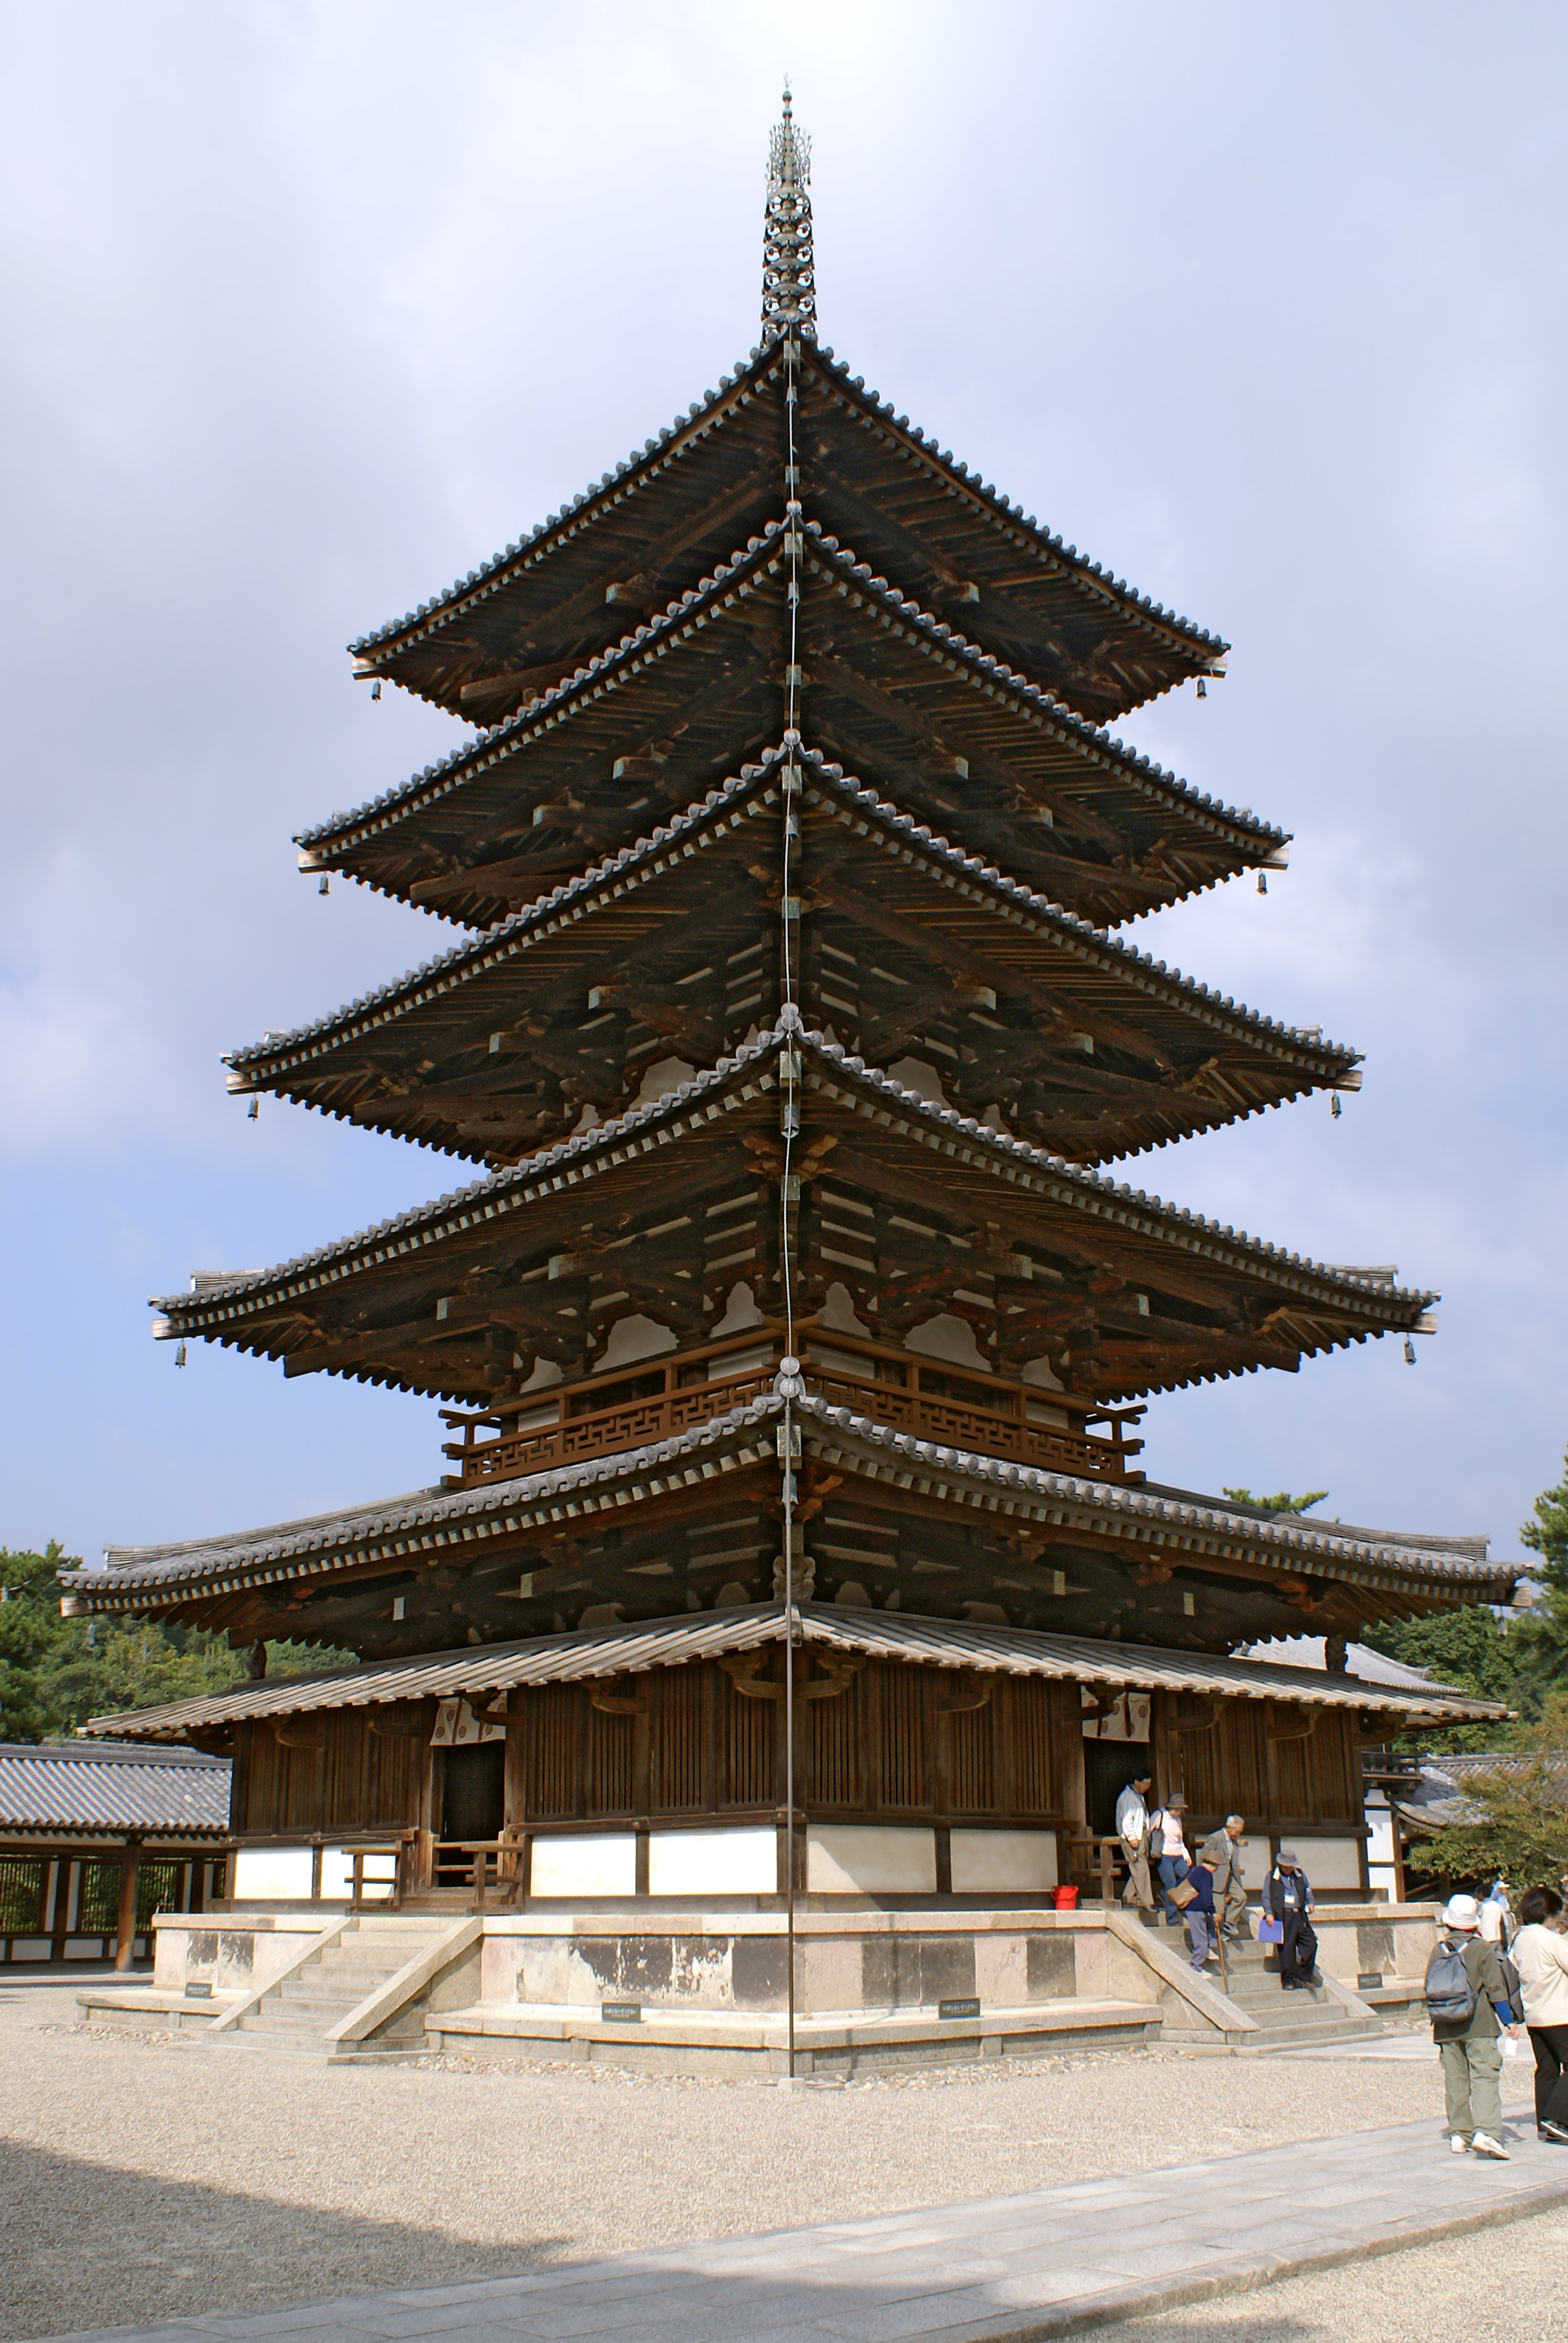
\includegraphics{pagoda}
}
\end{array}
\]

\end{frame}

\begin{frame}\frametitle{Maude's metalevel}

In Maude, key functionality of the universal theory $\mathcal{U}$ has 
been efficiently implemented in the functional module \texttt{META-LEVEL}:

\begin{itemize}
\item 
Maude \enfa{terms} are reified as elements of a data type \enfa{\texttt{Term}} in the 
module \texttt{META-TERM};

\item 
Maude \enfa{modules} are reified as terms in a data type \enfa{\texttt{Module}}
in the module \texttt{META-MODULE};

\item
operations  \texttt{upModule}, \texttt{upTerm}, \texttt{downTerm}, and others
allow \enfa{moving between reflection levels};
\end{itemize}

\end{frame}

\begin{frame}\frametitle{Maude's metalevel}
\begin{itemize}

\item
the process of \enfa{reducing a term} to canonical form using Maude's \texttt{reduce}
command is metarepresented by a built-in function \enfa{\texttt{metaReduce}};

\item
the processes of \enfa{rewriting a term} in a system module using Maude's
\texttt{rewrite} and \texttt{frewrite} commands are metarepresented by
built-in functions \enfa{\texttt{metaRewrite}} and \enfa{\texttt{metaFrewrite}};

\item
the process of \enfa{applying a rule} of a system module \enfa{at the top}
of a term is metarepresented by a built-in function \enfa{\texttt{metaApply}};
\end{itemize}

\end{frame}

\begin{frame}\frametitle{Maude's metalevel}

\begin{itemize}
\item
the process of applying a rule of a system module at any
position of a term is metarepresented by a built-in function \enfa{\texttt{metaXapply}};

\item
the process of \enfa{matching} two terms is reified by
built-in functions \enfa{\texttt{metaMatch}} and \enfa{\texttt{metaXmatch}};

\item
the process of \enfa{searching} for a term satisfying some conditions starting in
an initial term is reified by
built-in functions \enfa{\texttt{metaSearch}} and \enfa{\texttt{metaSearchPath}}; and

\item
\enfa{parsing} and \enfa{pretty-printing} of a term in a module, as well as key sort
operations such as comparing sorts in the subsort ordering of a signature, are
also metarepresented by corresponding built-in functions.
\end{itemize}

\end{frame}

\begin{frame}[fragile]\frametitle{Metalevel syntax}
\begin{itemize}
\item
Sorts and kinds are metarepresented as data in specific subsorts of the
sort \texttt{Qid} of quoted identifiers (i.e., terms starting with the
\texttt{'} character, like \texttt{'Nat}).

\item
Terms can be either:
\begin{itemize}
\item
Constants, which are quoted identifiers containing the constant�s name and its type
separated by a \texttt{.} (e.g., \texttt{'0.Nat}).

\item
Variables, which contain their name and type separated by a �:� (e.g., \texttt{'X:Nat}).

\item
A built term is constructed by applying an operator symbol (a \texttt{Qid}) to a list of terms
(e.g., \verb"'_+_['0.Zero, 'N:Nat]"):

{\codesize
\begin{verbatim}
  sort TermList .
  subsort Term < TermList .
  op _,_ : TermList TermList -> TermList
      [ctor assoc gather (e E) prec 120] .
  op _[_] : Qid TermList -> Term [ctor] .
\end{verbatim}
}

\end{itemize}
\end{itemize}
\end{frame}

\begin{frame}[fragile]\frametitle{Metalevel syntax}
\begin{itemize}
\item
For metarepresenting modules, we have the sort \texttt{Module}:

{\codesize
\begin{verbatim}
 op fmod_is_sorts_.____endfm : Header ImportList SortSet
       SubsortDeclSet OpDeclSet MembAxSet EquationSet -> Module
       [ctor gather (& & & & & & &)] .
\end{verbatim}
}

\item
The constructors for the sorts used above follow Maude syntax:

{\codesize
\begin{verbatim}
 op eq_=_[_]. : Term Term AttrSet -> Equation [ctor] .
 op ceq_=_if_[_]. : Term Term EqCondition AttrSet -> Equation
       [ctor] .
\end{verbatim}
}

\item
For example, we metarepresent \texttt{\col{eq [add1] 0 + N = N .}} as a term
of sort \verb"Equation":

{\codesize
\begin{verbatim}
eq '_+_['0.Zero, 'N:Nat] = 'N:Nat [label('add1)] .
\end{verbatim}
}

\end{itemize}
\end{frame}


\begin{frame}[fragile]\frametitle{Representing modules: Example at the object level}

{\small
\begin{verbatim}
fmod NSET is
 pr NAT .
 sort Set .
 subsort Nat < Set .

 op empty : -> Set [ctor] .
 op _,_ : Set Set -> Set [ctor comm assoc id: empty] .

 var N : Nat .
 var S : Set .

 op |_| : Set -> Nat .
 eq [s1] : | empty | = 0 .
 eq [s2] : | N, S | = s(| S |) .

 op empty? : Set -> Bool .
 eq [e1] : empty?(empty) = true .
 eq [e2] : empty?((N, S)) = false .
endfm
\end{verbatim}
}

\end{frame}

\begin{frame}[fragile]\frametitle{Representing modules: Example at the metalevel}

{\small
\begin{verbatim}
fmod 'NSET is
  including 'BOOL .
  protecting 'NAT .
  sorts 'Set .
  subsort 'Nat < 'Set .
  
  op '_`,_ : 'Set 'Set -> 'Set [assoc comm ctor id('empty.Set)] .
  op 'empty : nil -> 'Set [ctor] .
  op 'empty? : 'Set -> 'Bool [none] .
  op '|_| : 'Set -> 'Nat [none] .
  
  none
  
  eq 'empty?['empty.Set] = 'true.Bool [label('e1)] .
  eq 'empty?['_`,_['N:Nat,'S:Set]] = 'false.Bool [label('e2)] .
  eq '|_|['empty.Set] = '0.Zero [label('s1)] .
  eq '|_|['_`,_['N:Nat,'S:Set]] = 's_['|_|['S:Set]] [label('s2)] .
endfm
\end{verbatim}
}

\end{frame}

\begin{frame}[fragile]\frametitle{Representing modules: Example at the object level}

{\small
\begin{verbatim}
mod BLACKBOARD is
 pr NSET .

 vars N N' : Nat .
 var  S : Set .

 rl [add] : N, N', S => ((N + N') quo 2), S .
endm
\end{verbatim}
}

\end{frame}

\begin{frame}[fragile]\frametitle{Representing modules: Example at the metalevel}

{\small
\begin{verbatim}
mod 'BLACKBOARD is
  including 'BOOL .
  protecting 'NSET .
  sorts none .
  none
  none
  none
  none
  rl '_`,_['N:Nat,'N':Nat,'S:Set] => 
     '_`,_['S:Set,'_quo_['_+_['N:Nat,'N':Nat],'s_^2['0.Zero]]]
     [label('add)] .
endm
\end{verbatim}
}

\end{frame}

\begin{frame}[fragile=singleslide]
  \frametitle{Moving between levels}

{\small
\begin{verbatim}
  op upModule : Qid Bool ~> Module [special (...)] .
  op upSorts : Qid Bool ~> SortSet [special (...)] .
  op upSubsortDecls : Qid Bool ~> SubsortDeclSet [special (...)] .
  op upOpDecls : Qid Bool ~> OpDeclSet [special (...)] .
  op upMbs : Qid Bool ~> MembAxSet [special (...)] .
  op upEqs : Qid Bool ~> EquationSet [special (...)] .
  op upRls : Qid Bool ~> RuleSet [special (...)] .
  
\end{verbatim}
}

In all these (partial) operations
\begin{itemize}
\item
The first argument is expected to be a module name.

\item
The second argument is a Boolean, indicating whether we are interested also
in the imported modules or not.
\end{itemize}  
  
\end{frame}

\begin{frame}[fragile=singleslide]
  \frametitle{Moving between levels: Terms}

{\small
\begin{verbatim}
  fmod UP-DOWN-TEST is protecting META-LEVEL .
    sort Foo .
    ops a b c d : -> Foo .
    op f : Foo Foo -> Foo .
    op error : -> [Foo] .
    eq c = d .
  endfm

  Maude> reduce in UP-DOWN-TEST : upTerm(f(a, f(b, c))) .
  result GroundTerm: 'f['a.Foo,'f['b.Foo,'d.Foo]]

  Maude> reduce downTerm('f['a.Foo,'f['b.Foo,'c.Foo]], error) .
  result Foo: f(a, f(b, c))
  
  Maude> reduce downTerm('f['a.Foo,'f['b.Foo,'e.Foo]], error) .
  Advisory: could not find a constant e of 
            sort Foo in meta-module UP-DOWN-TEST.
  result [Foo]: error
\end{verbatim}
}

\end{frame}

\subsection{Descent functions}

\begin{frame}[fragile=singleslide]
  \frametitle{\texttt{metaParse}}
  
\begin{itemize}
\item
Its first argument is the representation in \texttt{META-LEVEL} of a module
$\mathcal{R}$, its second argument is a list of quoted identifiers, and the third one
is a type. 

\item
It tries to parse the given list of tokens as a term of the
given type in the module given as first argument.

\item
The constant anyType allows any component.

\item
If \texttt{metaParse} succeeds, it returns the metarepresentation of the parsed term.

\item
Otherwise, it returns, \texttt{noParse} or \texttt{ambiguity}.
\end{itemize}

{\small
\begin{verbatim}
  Maude> reduce in META-LEVEL : metaParse(upModule('BLACKBOARD, false), 
                                          '3 '`, '4 '`, '5, anyType) .

  result ResultPair: {'_`,_['s_^3['0.Zero],'_`,_['s_^4['0.Zero],
                            's_^5['0.Zero]]],'Set}
\end{verbatim}
}

\end{frame}

\begin{frame}[fragile=singleslide]
  \frametitle{\texttt{metaReduce}}
  
\begin{itemize}
\item
Its first argument is the representation in \texttt{META-LEVEL} of a \enfa{module} 
$\mathcal{R}$ and its second argument is the representation in \texttt{META-LEVEL}
of a \enfa{term} $t$.  

\item
It returns the metarepresentation of the normal form of $t$, using the 
equations in $\mathcal{R}$, together with the metarepresentation of its 
corresponding sort or kind.

\item
The reduction strategy used by \texttt{metaReduce} coincides with that
of the \texttt{reduce} command:
\end{itemize}

{\small
\begin{verbatim}
  Maude> reduce in META-LEVEL : metaReduce(upModule('NSET, false), 
               '|_|['_`,_['0.Zero,'s_['0.Zero],'s_['s_['0.Zero]]]]) .

  result ResultPair: {'s_^3['0.Zero],'NzNat}
\end{verbatim}
}

\end{frame}
  
\begin{frame}[fragile=singleslide]
  \frametitle{\texttt{metaRewrite}}

\begin{itemize}
\item
Its first two arguments are the representations in \texttt{META-LEVEL} 
of a module $\mathcal{R}$ and of a term $t$, and its third argument is 
a natural $n$.

\item
Its result is the representation of the \enfa{term obtained from $t$ after at most 
$n$ applications of the rules in $\mathcal{R}$} using the strategy of 
Maude's command \texttt{rewrite}, together with the metarepresentation 
of its corresponding sort or kind.
\end{itemize}

{\footnotesize
\begin{verbatim}
  Maude> reduce in META-LEVEL :
           metaRewrite(upModule('BLACKBOARD, false),
             '_`,_['s_^2['0.Zero], '_`,_['s_^3['0.Zero],
             '_`,_['s_['0.Zero], '0.Zero]]], 1) .
  result ResultPair: 
    {'_`,_['0.Zero,'s_^2['0.Zero],'s_^3['0.Zero]], 'Set}

  Maude> reduce in META-LEVEL :
           metaRewrite(upModule('BLACKBOARD, false),
             '_`,_['s_^2['0.Zero], '_`,_['s_^3['0.Zero],
             '_`,_['s_['0.Zero], '0.Zero]]], 5) .
  result ResultPair:
    {'s_^2['0.Zero], 'NzNat}
\end{verbatim}
}

\end{frame}


\begin{frame}\frametitle{The Maude system: Full Maude}
\begin{itemize}
\item
Full Maude is an extension of Maude implemented in Maude itself.

\item
It provides a more powerful and extensible module algebra than that available in Core Maude.

\item
It includes 
object-oriented modules (which can be parameterized) with support notation for objects,
messages, classes, and inheritance.

\item
Full Maude has an \enfa{explicit database} for modules, which allows the user to manipulate them.

\item
It uses the Loop Mode module, generating an input/output loop to interact with the user.

\item
The Loop Mode forces us to introduce commands and modules by \col{enclosing them in parentheses}.

\item
All the commands available in Core Maude are available in Full Maude, and executed at
the metalevel.

\end{itemize}
\end{frame}

\begin{frame}\frametitle{The Maude system: Full Maude}
\begin{itemize}
\item
Full Maude itself can be used as a basis for further extensions, by adding new functionality.

\item
It is possible both to change the syntax or the behavior of existing features, and to add new features.

\item
For example, we can add \enfa{new modules} and \enfa{new commands}.

\item
In this way Full Maude becomes a common infrastructure on top of which one can build tools.

\item
Examples of new applications are the Maude Declarative Debugger, the Real-Time Maude
tool, and the Constructor-based Inductive Theorem Prover.

\end{itemize}
\end{frame}

\begin{frame}\frametitle{Objectives}
\begin{itemize}
\item
We present here an extension of Full Maude to accept CafeOBJ specifications.

\item
We have defined the syntax of CafeOBJ modules, so it can be parsed.

\item
These modules are then translated (when possible) into Maude modules.

\item
We have also created new commands to work with the original CafeOBJ
modules.

\item
We use this as basis for extending other tools.
\end{itemize}
\end{frame}

\begin{frame}\frametitle{Translation}
\begin{itemize}
\item
We translate:
\begin{itemize}
\item
Modules with loose semantics as theories.

\item
Modules with tight semantics as modules.

\item
Importantions, sorts, subsorts, operators (and their attributes), and equations as themselves.

\item
Predicates as Boolean operators.

\item
Transitions as rules.

\item
Since Maude does not support parameterized theories, we translate this kind
of module as a parameterized module, showing a message.

\item
Similarly, we change the importation mode for theories to \texttt{including},
showing a message warning the user.
\end{itemize}
\end{itemize}
\end{frame}

%%%%%%%%%%%%%%%%%%%%%%%%%%%%%%%%%%%%%%%%%%%%%%%%%%%%%%%%%%%%%%%%%%%%%%%%%%%%%%%%%%%%%%%%
%%%%%%%%%%%%%%%%%%%%%%%%%%%%% CafeOBJ: Defining the syntax %%%%%%%%%%%%%%%%%%%%%%%%%%%%%
%%%%%%%%%%%%%%%%%%%%%%%%%%%%%%%%%%%%%%%%%%%%%%%%%%%%%%%%%%%%%%%%%%%%%%%%%%%%%%%%%%%%%%%%

\section{Defining the syntax}

\begin{frame}[fragile]\frametitle{CafeOBJ: Syntax}
\begin{itemize}
\item
The first thing we need to do is defining CafeOBJ syntax.

\item
We have to declare the sorts the constructors:

{\codesize
\begin{verbatim}
sorts @CafeMODULE@ @HiddenSortDecl@ @VisibleSortDecl@ @CafeOpDecl@
      @CafeImportDecl@ @CafeType@ @CafeTypeList@ @CafeSortList@
      @CafeSort@ @BehaviorEquationDecl@ @CafeDeclList@ @CafeEqDecl@
      @CafeVarDecl@ @CafeSubSortRel@ @CafeLDeclList@ @CafeModExp@
      @CafeParameter@ @CafeParameters@ @CafeInterface@ 
      @CafeViewDecl@ @CafeViewDeclList@ @CafeTransDecl@ 
      @CafeViewId@ @CafeViewIdList@ @ReductionDecl@ .
\end{verbatim}
}

\end{itemize}
\end{frame}

\begin{frame}[fragile]\frametitle{CafeOBJ: Syntax}
\begin{itemize}
\item
More specifically, we have sorts for:
\begin{itemize}
\item
Modules: \verb"@CafeMODULE@".

\item
Sorts: \verb"@VisibleSortDecl@".

\item
Variable declarations: \verb"@CafeVarDecl@".

\item
Equations: \verb"@CafeEqDecl@".

\item
Etc.
\end{itemize}

\item
We have also define all the subsort relations:
\begin{itemize}
\item
For types: \verb"subsort @CafeToken@ < @CafeSort@ < @CafeType@ ."

\item
For view identifiers: \verb"subsort @CafeModExp@ < @CafeViewId@ ."

\item
For indicating the modules are the data type to be introduced:\\
\texttt{subsort @CafeMODULE@ < \enfa{@Input@} .}

\item
Etc.

\end{itemize}
\end{itemize}
\end{frame}

\begin{frame}[fragile]\frametitle{CafeOBJ: Syntax}
\begin{itemize}
\item
The next step is defining the constructors.

\item
These constructors just follow the CafeOBJ syntax from the manual
(taking into account the latest changes).

\item
For example, modules are defined as follows:
\begin{itemize}
\item
For loose semantics:

{\codesize
\begin{verbatim}
  op mod*_{_} : @CafeInterface@ @CafeDeclList@ 
                -> @CafeMODULE@ [ctor] .
\end{verbatim}
}

\item
For tight semantics

{\codesize
\begin{verbatim}
  op mod!_{_} : @CafeInterface@ @CafeDeclList@ 
                -> @CafeMODULE@ [ctor] .
\end{verbatim}
}

\item
For views:

{\codesize
\begin{verbatim}
  op view_from_to_{_} : @CafeToken@ @CafeModExp@ @CafeModExp@
                 @CafeViewDeclList@ -> @CafeMODULE@ [ctor] .
\end{verbatim}
}
\end{itemize}

\item
Shortcuts for creating modules are translated into terms with this syntax.
\end{itemize}
\end{frame}

\begin{frame}[fragile]\frametitle{CafeOBJ: Syntax}
\begin{itemize}
\item
Importation modes are declared as follows:

{\codesize
\begin{verbatim}
  op protecting(_) : @CafeModExp@ -> @CafeImportDecl@ [ctor] .
  op extending(_) : @CafeModExp@ -> @CafeImportDecl@ [ctor] .
  op including(_) : @CafeModExp@ -> @CafeImportDecl@ [ctor] .
  op using(_) : @CafeModExp@ -> @CafeImportDecl@ [ctor] .
\end{verbatim}
}

\item
Equations have the following syntax:

{\codesize
\begin{verbatim}
  op eq_=_. : @CafeBubble@ @CafeBubble@ -> @CafeEqDecl@ [ctor] .
  op ceq_=_if_. : @CafeBubble@ @CafeBubble@ @CafeBubble@ 
                  -> @CafeEqDecl@ [ctor] .
\end{verbatim}
}

\end{itemize}
\end{frame}

\begin{frame}[fragile]\frametitle{CafeOBJ: Syntax}
\begin{itemize}
\item
Note the sort \verb"@CafeBubble@" used for the lefthand side, the
righthand side, and the condition.

\item
It indicates that they can be anything.

\item
It is used because these terms do not depend on the CafeOBJ syntax, but on the specific
syntax defined in the module.

\item
We have to parse these bubbles later to:
\begin{itemize}
\item
Check that the terms are defined with valid functions.

\item
Look for labels and attributes.

\item
Check that the equation is executable (no new variables are used in
the righthand side).
\end{itemize}
  
\end{itemize}
\end{frame}

\begin{frame}[fragile]\frametitle{Parsing}
\begin{itemize}
\item
When the user introduces a CafeOBJ modules, it is into Full Maude as a list
of \verb"Qid".

\item
For example, the module

{\codesize
\begin{verbatim}
mod! TALK {
  [Foo]

  op a : -> Foo {constr}
  var F : Foo

  op f : Foo -> Foo
  eq f(F) = a .
}
\end{verbatim}
}

\noindent
is read as:

{\codesize
\begin{verbatim}
'mod! 'TALK '`{ '`[ 'Foo '`] 'op 'a ': '-> 'Foo '`{ 'constr '`}
'var 'F ': 'foo
'op 'f ': 'Foo '-> 'Foo 'eq 'f '`( 'F '`) '= 'a '. '`}
\end{verbatim}
}

\end{itemize}
\end{frame}

\begin{frame}[fragile]\frametitle{Parsing}
\begin{itemize}
\item
Using the CafeOBJ syntax to (meta)parse it, we obtain

{\begin{verbatim}
'cmod!_`{_`}['CafeToken[''TALK.Qid],
'__['`[_`]['CafeToken[''Foo.Qid]],
'__['op_:`->_`{_`}.['CafeToken[''a.Qid],'CafeToken[''Foo.Qid],
    'constr.@CafeAttr@],
'__['var_:_.['neCafeTokenList[''F.Qid],'CafeToken[''Foo.Qid]],
'__['op_:_->_.['CafeToken[''f.Qid],'CafeToken[''Foo.Qid],
               'CafeToken[''Foo.Qid]],
'eq_=_.['CafeBubble['__[''f.Qid,''`(.Qid,''F.Qid,''`).Qid]],
               'CafeBubble[''a.Qid]]]]]]]
\end{verbatim}
}

\end{itemize}
\end{frame}

\begin{frame}[fragile]\frametitle{Parsing}
\begin{itemize}
\item
It is easy to translate the tokens.

\item
To translate the bubbles, we first create an intermediate module with
the importations, the variables, and the operator declarations in the module.

\item
In the CafeOBJ case, we have to extend the parsing with the variables defined
in the lefthand side of the equation/transition.

\item
Then, we use this module to solve the bubbles.

\item
In this case, we obtain \verb"'f['F:Foo]" from
\verb"'CafeBubble['__[''f.Qid,''`(.Qid,''F.Qid,''`).Qid]]".

\item
We have to check later that the executability restrictions hold.

\end{itemize}
\end{frame}

\begin{frame}[fragile]\frametitle{Parsing}
\begin{itemize}
\item
For example, predicates are parsed as Maude operators:

{\codesize
\begin{verbatim}
  ceq parseCafeDecl('pred_:_`{_`}.['CafeToken[T], T', T'''], 
                                PU, U, VDS, DB) = < PDR, nil, DB >
   if T4 := addSortToken(T') /\
      PDR := parseDecl('op_:_->_`[_`].['token[T], T4,
        'sortToken[''Bool.Qid], map2MaudeAttr(T''')], PU, U, VDS) .
\end{verbatim}
}

\noindent
where \verb"map2MaudeAttr" translates the CafeOBJ attributes:

{\codesize
\begin{verbatim}
  eq map2MaudeAttr(('constr.@CafeAttr@, TL)) = 'ctor.@Attr@, 
                                                map2MaudeAttr(TL) .
  eq map2MaudeAttr(('associative.@CafeAttr@, TL)) = 'assoc.@Attr@,
                                                map2MaudeAttr(TL) .
  ...
\end{verbatim}
}

\end{itemize}
\end{frame}

\begin{frame}[fragile]\frametitle{Parsing}
\begin{itemize}
\item
Transitions are translated as rules as follows:

{\codesize
\begin{verbatim}
ceq parseCafeDecl('trans_=>_.['CafeBubble[T], 'CafeBubble[T']], PU,
                    U, VDS, DB) = < PDR, nil, DB >
 if QIL := downQidList(T) /\
    VDS' := VDS opDeclSetFromQidList(QIL) /\
    T'' := cafeEqAtS2maudeEqAts(T') /\
    PDR := parseDecl('rl_=>_.['bubble[T],'bubble[T'']], PU, U, VDS') .
\end{verbatim}
}

\noindent
where \verb"opDeclSetFromQidList" extends the set of variables with the ones
declared on-the-fly on the lefthand side.

\end{itemize}
\end{frame}

\begin{frame}[fragile]\frametitle{After parsing}
\begin{itemize}
\item
Once we can introduce CafeOBJ modules into the database, we can use any
Maude command with them.

\item
Moreover, we can define our own commands to interact with these modules.

\item
For example, it might be interesting to define a command to show the
original module, since the Maude commands show the translated one.

\item
This is done by:
\begin{itemize}
\item
Extending the Full Maude syntax for commands.

\item
Defining rewrite rules dealing with this new commands.

\item
In this case we also need to define a new attribute to keep the original module,
since some translations cannot be undone (e.g.\ we do not know which Boolean
operators were originally predicates).
\end{itemize}

\end{itemize}
\end{frame}

%%%%%%%%%%%%%%%%%%%%%%%%%%%%%%%%%%%%%%%%%%%%%%%%%%%%%%%%%%%%%%%%%%%%%%%%%%%
%%%%%%%%%%%%%%%%%%%%%%%%%%%%%%%%%% INPUT %%%%%%%%%%%%%%%%%%%%%%%%%%%%%%%%%%
%%%%%%%%%%%%%%%%%%%%%%%%%%%%%%%%%%%%%%%%%%%%%%%%%%%%%%%%%%%%%%%%%%%%%%%%%%%

\subsection{Input}

\begin{frame}\frametitle{Accepted modules}
\begin{itemize}
\item
For some CafeOBJ modules the translation might not be accurate from the
semantics point of view.

\item
We use the syntax of the latest CafeOBJ release, so matching conditions
can be used in equations and transitions.

\item
We also accept statements using the \texttt{nonexec} attribute.

\item
A previous step of pre-processing allows the user to introduce \texttt{metadata}
information.
\end{itemize}
\end{frame}

\subsection{Example}

\begin{frame}\frametitle{Integration}
\begin{center}
{\Huge
\col{EXAMPLE}
}
\end{center}
\end{frame}

%%%%%%%%%%%%%%%%%%%%%%%%%%%%%%%%%%%%%%%%%%%%%%%%%%%%%%%%%%%%%%%%%%%%%%%%%%%%%%%%%
%%%%%%%%%%%%%%%%%%%%%%%%%%%%%%%%%% INTEGRATION %%%%%%%%%%%%%%%%%%%%%%%%%%%%%%%%%%
%%%%%%%%%%%%%%%%%%%%%%%%%%%%%%%%%%%%%%%%%%%%%%%%%%%%%%%%%%%%%%%%%%%%%%%%%%%%%%%%%

\section{Integration}

\begin{frame}\frametitle{Integration with other tools}
\begin{itemize}
\item
We can now proceed to integrate this extension with other tools built on top
of Full Maude.

\item
The easiest way to do it is just use with these tools the Maude modules
obtained after the translation.

\item
This is achieved by:
\begin{itemize}
\item
Extending the syntax of the tool with the one for CafeOBJ.

\item
Adding the rules for dealing with these specification by using a subsort
of the \texttt{CafeHandler}.
\end{itemize}

\end{itemize}
\end{frame}

\begin{frame}\frametitle{Integration with other tools}
\begin{itemize}
\item
This simple mechanism allows us to test and debug CafeOBJ specifications with
Maude tools.

\item
The test-case generator builds ground terms for the given function.

\item
The results can be checked by the user or against a correct specification.

\item
Declarative debugging builds a tree corresponding to an erroneous
computation.

\item
It asks questions about the subcomputations (stored in the nodes of the tree)
until the error is found.

\end{itemize}
\end{frame}

\begin{frame}[fragile]\frametitle{Integration with other tools}
\begin{itemize}
\item
Given the following specification:

{\codesize
\begin{verbatim}
mod! LIST {
  pr(NAT)
  [Nat < List]

  op nil : -> List {constr}
  op __ : List List -> List {constr assoc id: (nil)}

  var N : Nat
  var L : List

  op reverse : List -> List
  eq [r1] : reverse(nil) = 0 .
  eq [r2] : reverse(N L) = reverse(L) N .
}
\end{verbatim}
}

\end{itemize}
\end{frame}

\begin{frame}[fragile]\frametitle{Integration with other tools}
\begin{itemize}
\item
We can first generate test cases by selecting a coverage criterium.

{\codesize
\begin{verbatim}
Maude> (function coverage .)
Function Coverage selected
\end{verbatim}
}

\noindent
which indicates that all the calls to a given function must use all the
possible equations defining it.

\item
Then, we can test the \verb"reverse" function as follows:

{\codesize
\begin{verbatim}
Maude> (test reverse .)

1 test cases have to be checked by the user:
    1. The term reverse(0 0) has been reduced to 0 0 0

All calls were covered.
\end{verbatim}
}

\end{itemize}
\end{frame}

\begin{frame}[fragile]\frametitle{Integration with other tools}
\begin{itemize}
\item
Since it is not an expected result, we can debug it with the command:

{\codesize
\begin{verbatim}
Maude> (debug reverse(0) -> 0 0 .)
\end{verbatim}
}

\item
Maude builds the following tree, where the application of each equation has as children the
equations directly applied when executing it:

$$
\infer[\lab{r2}]{\texttt{reverse(0 0)}\rightarrow \texttt{0 0 0}}{
	\infer[\lab{r2}]{\texttt{reverse(0)}\rightarrow \texttt{0 0}}{
		\infer[\lab{r1}]{\texttt{reverse(nil)}\rightarrow \texttt{0}}{
			{}
		}
	}
}
$$
\end{itemize}
\end{frame}

\begin{frame}[fragile]\frametitle{Integration with other tools}
\begin{itemize}
\item
The tool asks the following questions:

{\codesize
\begin{verbatim}
Is this reduction (associated with the equation r2) correct?

reverse(0) -> 0 0

Maude> (no .)

Is this reduction (associated with the equation r1) correct?

reverse(nil) -> 0

Maude> (no .)
\end{verbatim}
}

\item
With these answers it finds the error:

{\codesize
\begin{verbatim}
The buggy node is:
reverse(nil) -> 0
with the associated equation: r1
\end{verbatim}
}
\end{itemize}
\end{frame}

\subsection{Example}

\begin{frame}\frametitle{Integration}
\begin{center}
{\Huge
\col{EXAMPLE}
}
\end{center}
\end{frame}

\section{Integration with the CITP}

\begin{frame}\frametitle{Integration with other tools}
\begin{itemize}
\item
We can also integrate other tools but rebuilt the interface to hide Maude
and use CafeOBJ syntax.

\item
It requires, in addition to the changes above, to add a new attribute distinguishing
the language we are using.

\item
Then, we have to redefine all (or most of) the commands provided by the tool to
use our syntax.
\end{itemize}
\end{frame}

\begin{frame}\frametitle{Integration with other tools}
\begin{itemize}
\item
For example, we have the Constructor-based Inductive Theorem Prover (CITP).

\item
It can prove properties on Maude specifications.

\item
These properties are described by means of equations, membership axioms, or rules
in Maude syntax.

\item
However, in our case we are interested on equations and transitions in
CafeOBJ syntax.

\item
Hence, we have to define rules in charge of processing this command.

\item
It is also necessary to define rules for errors.
\end{itemize}
\end{frame}

\begin{frame}[fragile]\frametitle{Integration with other tools}

The rule for introducing goals in CafeOBJ is defined as follows:

{\footnotesize
\begin{verbatim}
  crl [goal-Mod-cafe] :
      < O : X@Database | db : DB, input : ('goal_|-_[T, T']), output : nil,
                         default : ME, pTree : P, currentGoal : GID, showMod : B,
                         language : cafeobj, originalCafeModule : TL, Atts >
   => < O : X@Database | db : DB, input : nilTermList,
                         output : (if QIL == 'OK
                                   then QIL'
                                   else QIL
                                   fi), default : ME, pTree : P',
                         currentGoal : getDefaultGoalIndex(P'), showMod : B,
                         language : cafeobj, originalCafeModule : T1, Atts >
   if ME' := parseModExp(T) /\
      < DB' ; ME'' > := evalModExp(ME', DB) /\
      < T1 ; ODS ; M > := getTermModule(ME'', DB') /\
      isCafeMod?(T1) /\
      << DB'' ; P' ; QIL >> := procGoalsCafe(DB', ME'', T') /\
      QIL' := prettyPrintProofTreeCafe(P', DB', B, T1) '\n '\g
              'INFO: '\o 'an 'initial 'goal 'generated! .
\end{verbatim}
}
\end{frame}

\begin{frame}\frametitle{Integration with other tools}
\begin{itemize}
\item
The \texttt{\col{input}} is the same as the one for Maude specifications.

\item
The flag for \texttt{\col{language}} is \texttt{\col{cafeobj}}.

\item
We use the function \texttt{\col{isCafeMod}} to check whether it is a valid CafeOBJ.

\item
The command is processed with a new function \texttt{\col{procGoalsCafe}}, which
generates the goal updates the database.

\item
The goal is printed with the function \texttt{\col{prettyPrintProofTreeCafe}},
which generates CafeOBJ-like output.

\item
For this purpose we use the original CafeOBJ module, stored in the
\texttt{\col{originalCafeModule}} attribute.
\end{itemize}
\end{frame}

\begin{frame}[fragile]\frametitle{Integration with other tools}
\begin{itemize}
\item
Given a theory stating the existence of a sort:

{\codesize
\begin{verbatim}
mod* ELT {
 [Elt]
}
\end{verbatim}
}

\item
And a simple module specifying lists:

{\codesize
\begin{verbatim}
mod! LISTS(X :: ELT) {
  [List]
  op nil : -> List {constr}
  op __ : Elt.X List -> List {constr}
\end{verbatim}
}

\item
With composition of lists:

{\codesize
\begin{verbatim}
  op _@_ : List List -> List
  eq nil @ L2 = L2 .
  eq (E L1) @ L2 = E (L1 @ L2) . *** [metadata "CA-1"] .
\end{verbatim}
}
\end{itemize}
\end{frame}

\begin{frame}[fragile]\frametitle{Integration with other tools}
\begin{itemize}
\item
And a non-deterministic function that combines two different lists:

{\codesize
\begin{verbatim}
  op mix : List List -> List {comm}

  trans [m1] : mix(nil, L) => L .
  trans [m2] : mix(E L1, L2) => E mix(L1, L2) .
}
\end{verbatim}
}

\item
We can indicate that we are working with CafeOBJ specifications:

{\codesize
\begin{verbatim}
 Maude> (cafeOBJ language .)
 CafeOBJ selected as current specification language.
\end{verbatim}
}

\end{itemize}
\end{frame}

\begin{frame}[fragile]\frametitle{Integration with other tools}
\begin{itemize}
\item
And define goals with transitions:

{\codesize
\begin{verbatim}
Maude> (goal LISTS |- trans mix(L1:List, nil) => L1 ;)
====================== GOAL 1-1 ======================
< Module LISTS is concealed
...
end
,
	  trans mix(L1:List,nil)
	    => L1:List . >
unproved

INFO: an initial goal generated!
\end{verbatim}
}

\end{itemize}
\end{frame}

\begin{frame}[fragile]\frametitle{Integration with other tools}
\begin{itemize}
\item
Then we can use the standard commands to prove it:

{\codesize
\begin{verbatim}
Maude> (auto .)

INFO: Goal 1-1 was successfully proved
by applying tactic: SI CA CS TC IP

INFO: PROOF COMPLETED
\end{verbatim}
}

\end{itemize}
\end{frame}

\subsection{Example}

\begin{frame}\frametitle{Integration}
\begin{center}
{\Huge
\col{EXAMPLE}
}
\end{center}
\end{frame}

%%%%%%%%%%%%%%%%%%%%%%%%%%%%%%%%%%%%%%%%%%%%%%%%%%%%%%%%%%%%%%%%%%%%%%%%%%%%%%%%%
%%%%%%%%%%%%%%%%%%%%%%%%%%%%%%%%%% CONCLUSIONS %%%%%%%%%%%%%%%%%%%%%%%%%%%%%%%%%%
%%%%%%%%%%%%%%%%%%%%%%%%%%%%%%%%%%%%%%%%%%%%%%%%%%%%%%%%%%%%%%%%%%%%%%%%%%%%%%%%%

\section{Concluding remarks and future work}

\subsection{Concluding remarks}

\begin{frame}\frametitle{Concluding remarks}
\begin{itemize}
\item
We have implemented an extension of Full Maude to parse CafeOBJ specifications.

\item
The standard Maude commands, such as \texttt{reduce}, \texttt{rewrite},
\texttt{search}, and \texttt{modelCheck} can be used with these specifications.

\item
This extension eases the integration of CafeOBJ specification with any tool implemented
in top of Full Maude.

\item
We have shown how to integrate tools from the implementation point of view,
but we have to devote some time to check that we are using these tools
appropriately from the theoretical point of view.

\end{itemize}
\end{frame}

%\section{Future work}
%
%\begin{frame}\frametitle{Future work}
%\begin{itemize}
%\item
%
%\end{itemize}
%\end{frame}

%%%%%%%%%%%%%%%%%%%%%%%%%%%%%%%%%%%%%%%%%%%%%%%%%%%%%%%%%%%%%%%%%%%%%%%%%
%%%%%%%%%%%%%%%%%%%%%%%%%%%%%%%%%% END %%%%%%%%%%%%%%%%%%%%%%%%%%%%%%%%%%
%%%%%%%%%%%%%%%%%%%%%%%%%%%%%%%%%%%%%%%%%%%%%%%%%%%%%%%%%%%%%%%%%%%%%%%%%

%\section*{Thanks}

%\begin{frame}
%\Huge{\col{Thank you for your attention.}}
%\vspace{5ex}
%\Huge{\col{Questions?}}

%\end{frame}

\end{document}
